\section{Systemtest med kendt input}
I dette afsnit vil det samlede system testes, således det er muligt at undersøge, om systemet behandler dette input, som det forventes. På baggrund af disse målinger er det muligt at konkludere, hvorvidt systemet virker. 

\subsection{Beskrivelse}
For at teste signalerne fra accelerometrene indsendes to spændinger svarende til hvert deres output. Denne varieres over tid, således spændingen svarer til samlet grader mellem $90-180^{\circ}$. Derudover testes det om vinklen vil falde til $-200^{\circ}$ for hvert accelerometer, når spændingen svarende til $180^{\circ}$ overskrides. 

For at teste det samlede system med et kendt input benyttes en funktionsgenerator, således et $500~Hz$ sinussignal med en peak-peak-amplitude på $4~mV$ kan genereres. Sinussignalets frekvens og amplitude er nær ved, hvad der kan forventes af et filtreret EMG-signal. Outputtet fra sinussignalet er filtreret gennem det implementerede digitale lavpasfilter. 

Testen foretages over 10 sekunders måling og optages via mikrokontrolleren. Ud fra disse målinger, er det muligt at teste effekten af systemets blokke, når de er sammensat ved at sammenligne input og output af det samplede sinussignal samt spændingerne for acclerometrene omregnet til en samlet vinkel. Resultaterne fra målingerne visualiseres i MATLAB. 


\subsection{Resultater af test}
Fra testen plottes og visualiseres systemets input af det samplede sinussignal, output fra det opsamlede digital filtrerede signal, samt spændingen fra de to accelerometre, der er omregnet til en samlet vinkel ved lineær interpolation. Derudover er det opsamlede digitale output, som er behandlet i EMG-algortimen, plottet. Resultaterne fremgår af \autoref{fig:test_kendtinput}. 

\begin{figure}[H]
\centering
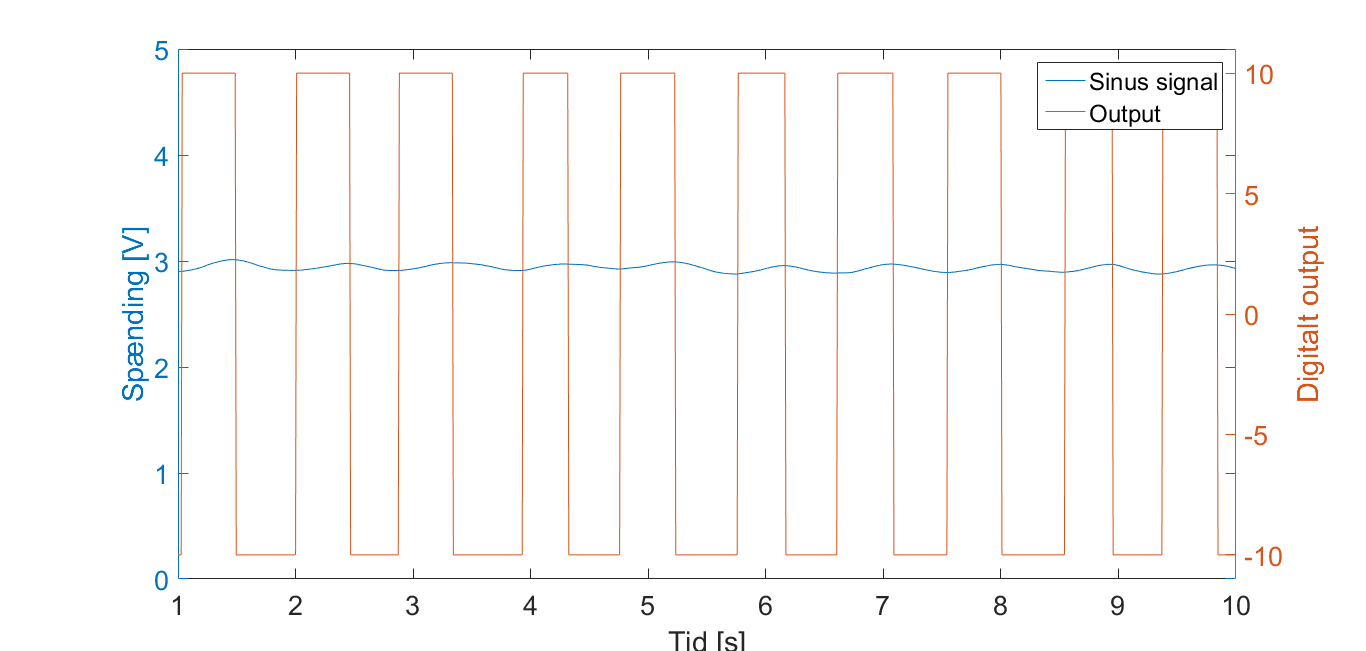
\includegraphics[width=0.7\textwidth]{figures/kontrol_test_sinus}
\caption{På den øverste figur illustreres den samlede vinkel over tid. Det fremgår af grafen, at vinklen er stigende fra $90^{\circ}$ til $175^{\circ}$, hvorefter vinklen falder markant til $-115^{\circ}$. Dette skyldes en overskridelse af spædningen for accelerometeret svarende til $180^{\circ}$.
På den midterste figur illustrerer den blå graf det opsamlede inputsignal, svarende til en sinus på $500~Hz$ med en $V_{pp}$ på $4~mV$. Den røde graf illustrerer det samplede sinussignal med et implementeret digitalt lavpasfilter, disse værdier er målt i spænding. 
På den nederste figur illustreres signalets digitale output. Signalet går fra $+10$ ved stigende muskelaktivitet til $-10$ ved en faldende muskelaktivitet. Grafen går i $0$, når en overskridelse af en vinkel $180^{\circ}$ opnås.}
\label{fig:test_kendtinput}
\end{figure}

På baggrund af målingerne for den øverste figur på \autoref{fig:test_kendtinput} fremgår det, at en indsendt stigende spænding svarende til $90-175^{\circ}$, får den samlede vinkel til at stige. Ved en vinkel på $175^{\circ}$ overskrider det ene accelerometer dens maks spænding, hvorfor vinklen daler markant på $1~ms$ til $-115^{\circ}$. Dette burde ifølge den implementerede kode gå ned til en vinkel på $-200^{\circ}$ ved overskridelse af ét accelerometeres grænse spændinger. 
Vinklen som ikke når $-400^{\circ}$ er en indikatior for, at det ene accelerometers spænding har været indenfor dens grænser, mens det andet accelerometer har overskredet dens grænser. Hertil kan det ses, at det ene accelerometer har haft indsendt en spænding svarende til $85^{\circ}$, mens det andet accelerometer har haft en spænding der har overskredet grænsen og derfor har en vinkel på $-200^{\circ}$.
Det fremgår af den midterste samt nederste figur på \autoref{fig:test_kendtinput}, at der ses en sammenhæng mellem det opsamlede digital filtrerede sinussignal og det opsamlede outputsignal. Ved et stigende sinussignal vil outputsignalet indikerer $10$, hvilket svarer til en stigning af sinussignalet. Ved fald af sinussignalet vil outputsignalet indikerer et fald og dermed ligge i $-10$.

På den nederste figur på \autoref{fig:test_kendtinput} fremgår det, at efter outputsignalet har befundet sig i $-10$ ved 9 sekunder, stiger outputsignalet efterfølgende til $0$. Dette er grundet, at de samlede grader har overskredet én eller flere grænser, og derved fungerer EMG-algorimten ikke, hvilket illustreres med at outputsignalet går i $0$.

Der er yderligere foretaget en test af det samlede forsinkelse på systemet. Denne test blev udført på samme måde som i \autoref{sec:lavpas_test} \autoref{sec:mavg_test}. Resultaterne for forsinkelse blev målt til $832~\mu~s$ for det samlede system. 